\documentclass[a4paper,fleqn]{jsarticle}

\usepackage[dvipdfmx]{graphicx}
\usepackage{bm}
\usepackage{amsmath,amssymb,amsfonts}
\usepackage[dvipdfmx]{color}

\usepackage{url}
\usepackage{okumacro}

 %ハイパーリンクの設定
\usepackage[dvipdfmx,colorlinks=true, bookmarks=true,
bookmarksnumbered=true, bookmarkstype=toc, linkcolor=blue,
urlcolor=blue, citecolor=blue]{hyperref}

\usepackage{pxjahyper}

%% source code
%\usepackage{listings,jlisting}
%\renewcommand{\lstlistingname}{source code}
%\lstset{language=C++,
%basicstyle=\ttfamily\small,
%  commentstyle={ \color[cmyk]{1,0.4,1,0}},
%  classoffset=1,
%  keywordstyle={\bfseries \color[cmyk]{0,1,0,0}},
%  stringstyle={\ttfamily \color[rgb]{0,0,1}},
%  frame=tRBl,
%  framesep=5pt,
%  showstringspaces=false,
%  numbers=left,
%  stepnumber=1,
%  numberstyle=\small,
%  tabsize=2,
%}

\renewcommand{\figurename}{Fig.}
\renewcommand{\refname}{Reference}
\renewcommand{\contentsname}{Contents}
\renewcommand{\abstractname}{Abstract}

%layout 
\setlength{\topmargin}{-20mm}
\setlength{\textheight}{25.5cm}
\setlength{\oddsidemargin}{0pt}
\setlength{\evensidemargin}{0pt}

\pagestyle{headings}

%date 
\def\today{%
  \ifcase\month\or
                Jan.\or Feb.\or Mar.\or Apr.\or May.\or Jun.\or
                Jul.\or Aug.\or Sep.\or Oct.\or Nov.\or Dec.
  		\fi\hspace{0.0em} 
%  \ifnum\month<10 0\fi\the\month/%
  \ifnum\day<10 0\fi\the\day, 
  \the\year%
}

%%%%%%%%%%%%%%%%%%%%%%%%%%%%%%%%%%%%%%%%%%%%%%%%%%%%%%%
%%%% end preamble
%%%%%%%%%%%%%%%%%%%%%%%%%%%%%%%%%%%%%%%%%%%%%%%%%%%%%%%%%
%%%%%%%%%%%%%%%%%%%%%%%%%%%%%%%%%%%%%%%%%%%%%%%%%%%%%%%%%%%


\begin{document}

\thispagestyle{plain}
%% report title
\begin{flushleft}
\begin{Large}
OpenFOAMの境界条件の取扱い方について
\end{Large}
\end{flushleft}

%% author
\begin{flushright}
\西暦
作成 2016/03/10\\
\end{flushright}


\begin{abstract}
CFDコードOpenFOAMで境界条件がどのように扱われているかについて説明する。
\end{abstract}

%\tableofcontents

\hrulefill
%%%%%%%%%%%%%%%%%%%%%%%%%%%%%%%%%%%%%%%%%%%%%%%%
%%%  本文
%%%%%%%%%%%%%%%%%%%%%%%%%%%%%%%%%%%%%%%%%%%%%%%



\section{fixedValue, fixedGradientについて}
これらの境界条件の説明については\cite{Nozaki}が詳しい。本節でもこれを元
にして説明を行う。

Fig.\ref{fig:cell}に示すような1次元の計算セルでの離散化を考える。セル中
心Pと境界Bでの境界条件を考える。セル中心Pと境界Bの間の距離を$\Delta x$と
する。
%%% Figure
 \begin{figure}[htbp]
  \begin{center}
   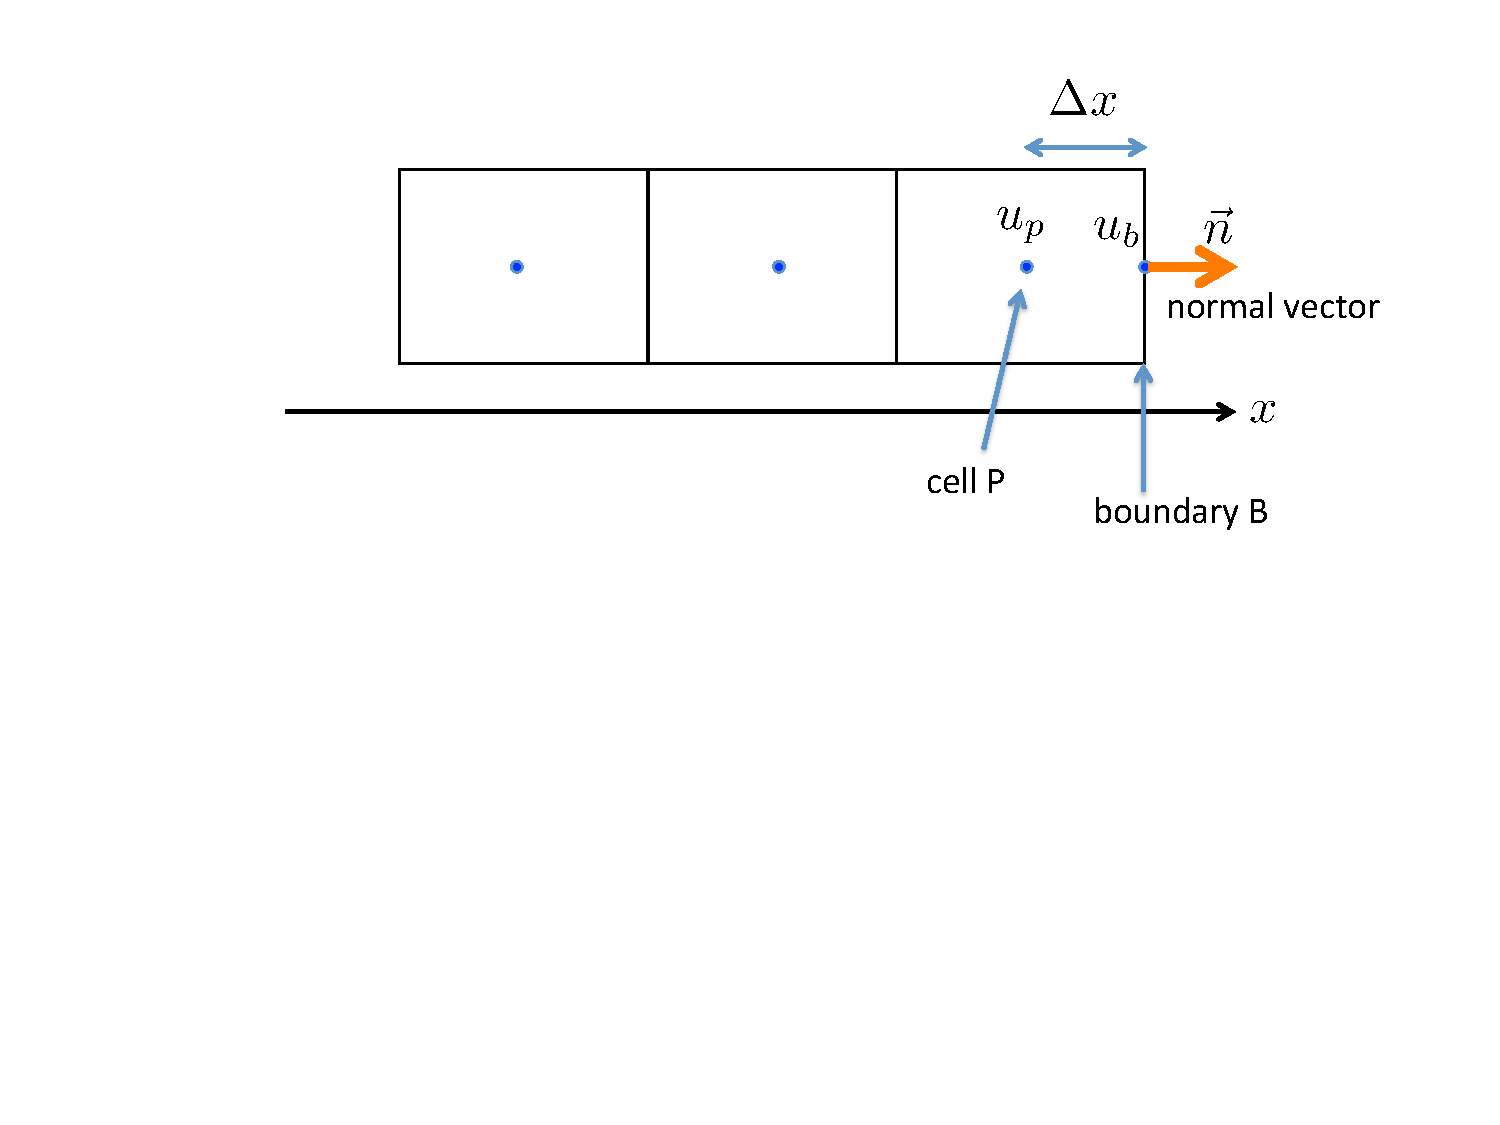
\includegraphics[scale=0.4]{Fig/cell.pdf}
   \caption{1D mesh}
   \label{fig:cell}
  \end{center}
\end{figure}

変数$u$の移流拡散方程式を有限体積法により解くものとする。$\nabla \cdot \nabla u$お
よび$\nabla \cdot u$は以下のように離散化される。

\begin{align}
 & \int \nabla \cdot (\nabla u) dV=\int \nabla u \cdot \bm{n}dS
 \approx \sum \nabla u \cdot \bm{n} S_f \\
 & \int \nabla \cdot u dV=\int u \cdot \bm{n} dS \approx \sum u \cdot
 \bm{n} S_f
\end{align}
$S_f$はfaceでのセル面積である。これらの式から境界での$\nabla u$および$u$
の値が必要であることが分かる。

\subsection{fixedValueについて}
はじめにDirichlet条件であるfixedValueについて考える。境界条件として

\begin{align}
 u_b=a
\end{align}
を考える。$a$は定数とする。

まず$\nabla u$の境界条件について考える。
\begin{align}
 & \nabla u|_{boundary}\cdot \bm{n}=\frac{u_b-u_p}{\Delta x} 
 = -\frac{1}{\Delta x} u_p + \frac{1}{\Delta x} a \label{eq:BC1}
\end{align}

OpenFOAMでは(\ref{eq:BC1})の係数がそれぞれgradinetInternalCoeff,
gradientBoundaryCoeffとして扱われる。InternalCoeffはセル内部の未知数に対
する係数であり,連立1次方程式の係数行列に反映される。一方BoundaryCoeffは
境界の値そのものであり,連立1次方程式の右辺ベクトルに反映される。

\begin{align}
& gradientInternalCoeff=-\frac{1}{\Delta x} \\
& gradientBoundaryCoeff=\frac{1}{\Delta x}a
\end{align}


つぎに$u$の境界条件について考える。ここではすでに$u|_{boundary}=a$として値は分かっている。
これらの値はvalueInternalCoeff, valueBoundaryCoeffとして扱われる。

\begin{align}
& valueInternalCoeff=0 \\
& valueBoundaryCoeff=a 
\end{align}


\subsection{fixedGradientについて}
Neumann条件であるfixedGradientについて考える。境界条件として

\begin{align}
 \nabla u|_{boundary} \cdot \bm{n}=b
\end{align}
を考える。$b$は定数。

$\nabla u$について考えると,すでに境界条件として与えられているので

\begin{align}
& gradientInternalCoeff=0 \\
& gradientBoundaryCoeff=b
\end{align}

つぎに$u$の条件を考える。
\begin{align}
 \nabla u\cdot \bm{n}=\frac{u_b-u_p}{\Delta x}=b
\end{align}
より
\begin{align}
 u_b=u_p+b\Delta x
\end{align}
よって
\begin{align}
& valueInternalCoeff=1 \\
& valueBoundaryCoeff=b\Delta x 
\end{align}


\section{mixedについて}
Robin条件であるmixedについて考える。境界条件として
\begin{align}
 \alpha u_b +(1-\alpha)\nabla u|_b \cdot \bm{n} \Delta x=\alpha a + (1-\alpha)b
\end{align}
を考える。ここで$\alpha$は重み係数,$u_{ref}=a,\nabla u_{ref}\cdot \bm{n}=b$は定数とする。
$a,b$の値はOpenFOAMではそれぞれrefValue, refGradとして扱われる量である。
$\alpha$はvalueFracとして扱われる。

\begin{align}
 \nabla u|_b\cdot \bm{n}=\frac{u_b-u_p}{\Delta x}
\end{align}
より
\begin{align}
 & \alpha u_b+(1-\alpha)(u_b-u_p)=\alpha a+(1-\alpha)b \\
 & u_b=(1-\alpha)u_p+\alpha a +(1-\alpha)b\Delta x \label{eq:mixed}
\end{align}

$\nabla u|_b \cdot \bm{n}$について考える。
\begin{align}
 & \nabla u|_b \cdot \bm{n}=\frac{u_b-u_p}{\Delta x} \\
 & =\frac{-\alpha}{\Delta x}u_p +\frac{\alpha a}{\Delta x} +(1-\alpha)b
\end{align}
であるから
\begin{align}
& gradientInternalCoeff=\frac{-\alpha}{\Delta x}\\
& gradientBoundaryCoeff=\frac{\alpha a}{\Delta x} +(1-\alpha)b
\end{align}

つぎに$u_b$について考えると,
\begin{align}
& u_b=(1-\alpha)u_p+\alpha a +(1-\alpha)b\Delta x
\end{align}
より
\begin{align}
& valueInternalCoeff=(1-\alpha) \\
& valueBoundaryCoeff=\alpha a +(1-\alpha)b\Delta x
\end{align}

\subsection{mixedの使用例としてのwallHeatTransfer}
熱伝達係数$h$を指定した壁面熱伝達の境界条件wallHeatTransferではmixedを使っ
て,実装されている。mixedを用いた具体例として説明する。

Fig.\ref{fig:wallheat}に壁面熱伝達の模式図を示す。流体側の壁面隣接セル内
部の温度を$T_i$,壁面温度を$T_w$,外部の代表温度を$T_{inf}$とする。流体
から壁面への熱流束$q_{in}$は流体の熱伝導度$k$とセルサイズ$\Delta x$より
以下のように書ける。

\begin{align}
q_{in}=k\frac{T_i-T_w}{\Delta x} 
\end{align}
一方壁面から外部への熱流束$q_{out}$は熱伝達係数$h$を用いて
\begin{align}
 q_{out}=h(T_w-T_{inf})
\end{align}

$q_{in}=q_{out}$より$T_w$についての整理すると
\begin{align}
 T_w&=\frac{\frac{k}{\Delta x}T_i+h T_{inf}}{\frac{k}{\Delta x}+h} \\
 &=\frac{\frac{k}{h\Delta x}T_i+T_{inf}}{1+\frac{k}{h\Delta x}}
\end{align}
%
これが温度の境界条件となる。(\ref{eq:mixed})に示したmixedの境界での値
$u_b$の式と比較すると,以下のように係数を設定することでmixedを用いてこの
境界条件を実装できることが分かる。

\begin{align}
 & 1-\alpha=\frac{k/h\Delta x}{1+k/h\Delta x} \\
 &\alpha a=\frac{T_{inf}}{1+k/h\Delta x}\\
 &b=0 
\end{align}

上式から
\begin{align}
 & a=T_{inf} \label{eq:a} \\
 &b=0 \label{eq:b} \\
 &\alpha=\frac{1}{1+k/h\Delta x} \label{eq:alpha}
\end{align}
となる。

wallHeatTransferの実装をみると(OpenFOAM-2.3.x)

 \begin{screen}
  \begin{verbatim}
  refValue() = Tinf_;
  refGrad() = 0.0;
  \end{verbatim}
 \end{screen}

 \begin{screen}
  \begin{verbatim}
  valueFraction() =
        1.0/
        (
            1.0
          + turbModel.kappaEff(patchi)*patch().deltaCoeffs()/alphaWall_
        );
  \end{verbatim}
 \end{screen}
となっており,(\ref{eq:a})-(\ref{eq:alpha})となるように実装されていることが
分かる。ここでkappaEff(patchi)が熱伝導度,deltaCoeffs()が$\Delta x$の逆
数,alphaWall\_が熱伝達係数をそれぞれ表している。
 
 \begin{figure}[htbp]
  \begin{center}
   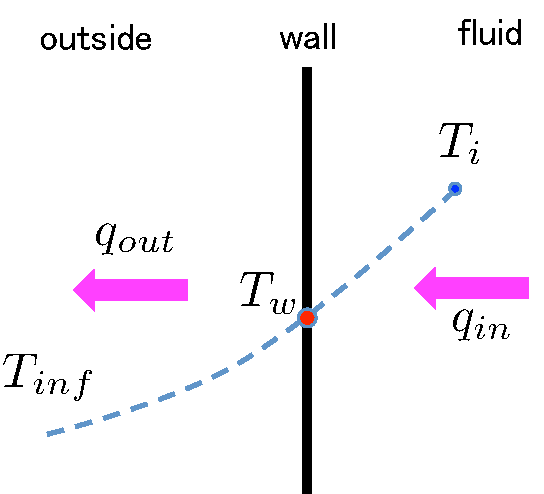
\includegraphics[scale=0.6]{Fig/wallheat.pdf}
   \caption{Wall heat transfer}
   \label{fig:wallheat}
  \end{center}
\end{figure}


%% reference
\begin{thebibliography}{99}
\bibitem{Nozaki} F. Nozaki, OpenFOAM 空間の離散化と係数行列の取り扱い, \url{http://www.slideshare.net/fumiyanozaki96/openfoam-32087641}

\end{thebibliography}



\end{document}
